% Appendix A -- methodology and implementation notes lifted out of the 8-page
% body. Every subsection here is pointed at by a \ref from Sections 1-4.
\section{Methodological and Implementation Details}
\label{app:methods}

\begin{figure*}[t]
  \centering
  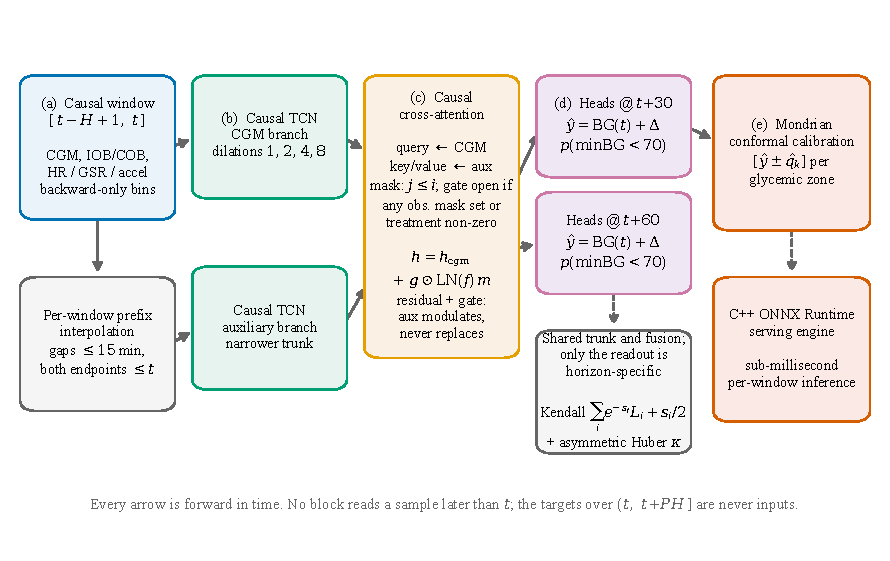
\includegraphics[width=0.9\textwidth]{fig1_architecture.pdf}
  \caption{CausalCGM-MT. (a)~A closed causal window feeds (b)~two causal TCN
  trunks, fused by (c)~cross-attention masked both temporally and by auxiliary
  availability, read out by (d)~per-horizon residual regression and nadir
  classification heads under a Kendall-weighted objective with the asymmetric
  hypoglycemia penalty, and deployed through (e)~Mondrian conformal calibration
  and a C++ ONNX engine. No block reads a sample later than $t$.}
  \label{fig:arch}
\end{figure*}

\subsection{Scope and Relation to Prior Work}
\label{sec:appendix_scope}

A user's tolerance for spurious alerts is finite, and the literature
systematically under-weights it. Alarm fatigue is a documented failure mode of
clinical monitoring in general~\citep{cvach2012monitor} and of diabetes devices
in particular~\citep{shivers2013turn}: users who receive too many spurious alerts
become less likely to respond to them, and an alert that is ignored protects
no one. A forewarning
system therefore has to be evaluated in the unit the patient experiences: false
alarms per day at a usable operating point, and how much warning a true alert
actually provides, not only in the units that are convenient to compute.

The multitask framing this paper builds on is not ours. \citet{fang2026glucose}
introduced MT-HypoNet, which couples continuous glucose forecasting to
hypoglycemia forewarning through a shared representation, and validated it on a
retrospective multicentre cohort of 1{,}662 patients spanning type~1 and type~2
diabetes, together with a prospective perioperative cohort of 36 further
patients, a scale of clinical evidence this work does not
approach. The statistically guided soft-label strategy for the hypoglycemia
boundary is likewise theirs. What we contribute is orthogonal to that evidence
and complementary to it. More specifically, the multitask formulation is adopted,
and the questions we ask are whether it can be trained without lookahead leakage, whether its
forewarning score can be given conditional coverage guarantees, and whether the
resulting artefact can be served with verified train/serve parity. Those are
engineering and evaluation questions, and answering them on a twelve-subject
public benchmark is a different exercise from establishing clinical
generalisation on 1{,}662 patients.

\subsection{The Auxiliary-Validity Defect}
\label{sec:appendix_aux_validity}

A window counts as
auxiliary-valid when, somewhere in its history, \emph{any} observation mask
among the streams in use is set or a mask-free treatment channel in use
(delivered insulin, insulin or carbohydrate on board, logged carbohydrate) is
non-zero. An earlier version read validity from the heart-rate mask alone. The 2020
OhioT1DM subjects wore an Empatica device that reports no heart rate, so that
channel is identically zero across all of their windows, the cross-attention was
fully masked, and the ``multimodal'' model was the CGM-only model for half the
cohort while continuing to report itself as multimodal. The same defect collapsed every modality-ablation arm that excluded
heart rate onto bit-identical numbers. We record the fraction of timesteps at
which the gate is open in every results file, and warn at training time when it
is zero.

\subsection{Note on the Kendall Weighting}
\label{sec:appendix_kendall}

Kendall et al.\ derive Equation~\ref{eq:kendall} as a Gaussian
maximum-likelihood objective in which $e^{-s_i}$ is a reciprocal noise variance
with a defined unit. Two departures are worth stating. The first is
presentational: under $s_i = \log \sigma_i^2$ their objective is
$\tfrac{1}{2}e^{-s_i}\mathcal{L}_i + \tfrac{1}{2}s_i$, and we drop the
$\tfrac{1}{2}$ on the loss term. A uniform factor on every task rescales the
whole objective and is absorbed by the learning rate, leaving the minimiser in
$s_i$ unchanged, so Equation~\ref{eq:kendall} is their objective up to that
constant. The second is substantive: neither of our terms meets the Gaussian
premise. The regression
loss is an asymmetric Huber whose weights depend on the reference value
(Equation~\ref{eq:asym}), so it is not the log-likelihood of any fixed noise
model and its implied density changes with $\kappa$; the classification loss is
a soft-label cross-entropy, whose corresponding derivation gives a different
form again. Treating the $s_i$ as commensurable uncertainties across the two is
therefore an analogy, not a probabilistic identity, and we do not claim the
learned $s_i$ estimate anything physical.

What the form does provide is a stable, scale-free way to combine terms whose
magnitudes differ by orders of magnitude and drift during training, with a
$\tfrac{1}{2} s_i$ penalty that stops the optimiser from driving either weight
to zero. Section~\ref{sec:ablation_a} measures this against a fixed
$\lambda = 1$ and finds the difference small and horizon-dependent. Read
Equation~\ref{eq:kendall}, then, as a well-behaved parameterisation of a
hyperparameter rather than a principled uncertainty model: a reader who prefers
the fixed-$\lambda$ arm loses little, and the value of the learned form is that
it removes a knob that would otherwise need re-tuning per cohort, horizon set
and class prior.

\subsection{Conformal Construction: Proof and Conventions}
\label{sec:appendix_conformal_method}

\paragraph{Zone conventions.} The brackets of
$\zone{1} = [0, 70)$, $\zone{2} = [70, 180]$, $\zone{3} = (180, \infty)$ follow
the clinical convention: both 70 and 180 lie inside the euglycemic band, so
$\zone{1} \cup \zone{2} \cup \zone{3} = [0, \infty)$ with the three pairwise
disjoint. In other words, every glucose value belongs to exactly one zone,
including the boundaries themselves. The same convention is implemented in
\texttt{clinical\_stratum}, where a non-finite value returns no stratum at all
rather than defaulting into $\zone{2}$.

\paragraph{Why the zone cannot be read from $\hat{y}$.} The taxonomy is a
function of the \emph{target}, which is unknown at inference. Mondrian conformal
is exactly valid for an observable taxonomy; assigning the zone from $\hat{y}$
and applying that zone's quantile is a heuristic that fails hardest where it is
needed: a true 60~mg/dL that the model reads as 100 receives the narrow
euglycemic width. Equation~\ref{eq:mondrian} instead emits the convex hull of the
label-conditional region, where zone $k$ contributes iff
$\operatorname{dist}(\hat{y}, \zone{k}) \le \hat{q}_k$.

\paragraph{The oracle-coverage guarantee.} This yields a two-line proof: if the true $y$ lies in $\zone{k}$ with
$|y - \hat{y}| \le \hat{q}_k$, then
$\operatorname{dist}(\hat{y}, \zone{k}) \le |y - \hat{y}| \le \hat{q}_k$, so zone $k$
is reachable and the emitted half-width is at least $\hat{q}_k$; hence $y$ is
covered. \emph{The emitted interval covers $y$ whenever the oracle interval, the
one built from the true and unobservable zone, would have.} A stratum with fewer
than $\lceil (1-\alpha)/\alpha \rceil$ calibration points cannot certify the
level at all and falls back to the pooled quantile with an explicit log record,
carrying the marginal guarantee rather than a conditional one.

\subsection{Deployment Path and Train/Serve Parity}
\label{sec:appendix_deployment}

The trained network is exported to ONNX behind a numerical-parity and causality
gate, and served by a standalone C++ ONNX Runtime~\citep{onnxruntime} binary with
no Python in the loop. Feature construction is reimplemented in C++ and verified
against the Python path element by element, because a graph-level parity check
cannot see it: a divergence in the hand-written feature code is train/serve skew,
in which the deployed model receives different inputs from the ones it was
trained on while every export test still passes.
The C++ path is verified for the CGM channels only: the runner implements no
auxiliary feature path and serves a fusion graph with its auxiliary input zeroed
and the presence gate closed, which is exactly the CGM-only computation, and
the element-wise parity check runs on a CGM-only demonstration graph. Serving
the fusion model with live auxiliary streams is not implemented.
Section~\ref{sec:edge} reports what that stack costs to run. We describe it as a
deployment path rather than as an embedded implementation: the binary targets a
general-purpose CPU, and porting it to constrained silicon is out of scope
here.

\subsection{Runtime Overhead of the Serving Stack}
\label{sec:edge}

\begin{figure*}[t]
  \centering
  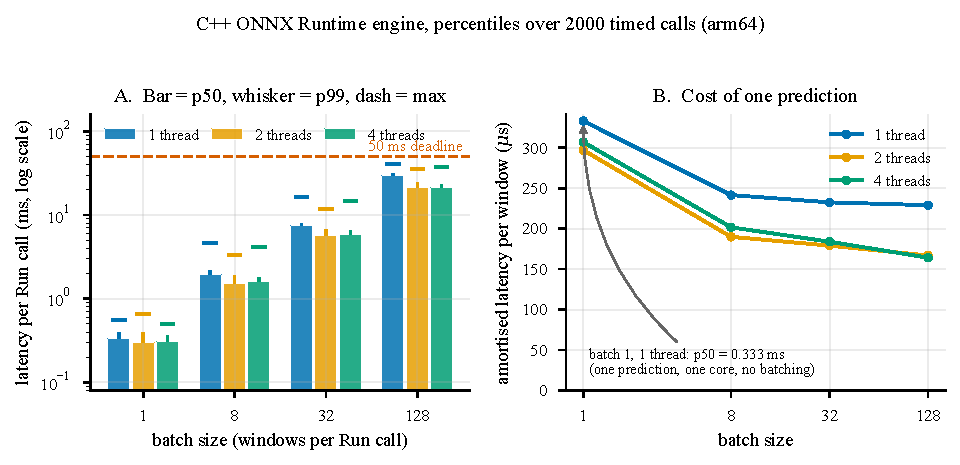
\includegraphics[width=\textwidth]{fig6_edge_latency.pdf}
  \caption{C++ ONNX Runtime engine. (A)~Per-call latency against a
  $\NumEdgeDeadline$~ms deadline; bar is p50, whisker p99, dash the observed
  maximum. (B)~Amortised cost of a single prediction. Percentiles are as
  reported by the runner over its own timed calls.}
  \label{fig:edge}
\end{figure*}

\paragraph{What this section does and does not establish.} We state the scope
first to prevent a likely misreading. These measurements were taken on an \NumEdgeCPU{} ($\NumEdgeCores$ cores), a
desktop-class processor. They are \emph{not} evidence that CausalCGM-MT meets a
real-time budget on an insulin pump, a Cortex-M microcontroller, or a
phone-tethered wearable, and we make no such claim. What they establish is
narrower: the deployment path we ship (ONNX export, a standalone C++ ONNX Runtime
binary, and a C++ reimplementation of the feature construction) adds negligible
overhead of its own. A future port to target silicon is therefore a question
about that silicon rather than about accumulated inefficiency in the serving
stack.

The graph benchmarked has the architecture of the \NumEdgeGraph{} model reported in
Table~\ref{tab:sota_ph30}: the dual-trunk network with cross-attention and both
horizon heads, not a reduced stand-in. The latency artefact records the graph's
file path and parameter count but not its weights, so these timings concern the
architecture and are not shown to belong to the Table~\ref{tab:sota_ph30}
checkpoint. It runs against ONNX Runtime~1.23.2 in
the Release build, timing the \texttt{Run} call alone; the chip is recorded in
the artefact the numbers are read from rather than named here by hand. A single
window costs $\NumEdgePFifty$~ms at the median and $\NumEdgePNinetyNine$~ms at
p99 on one thread, with a worst observed call of $\NumEdgeMax$~ms. Feature
construction adds $\NumEdgeFeatureUs$~$\mu$s per window, roughly three orders of
magnitude below the inference call. This is the specific overhead result the
section reports: the hand-written C++ feature path that must match the training
pipeline bit for bit costs essentially nothing to run. Batching
amortises to $\NumEdgeBestPerWindowUs$~$\mu$s per window at batch
$\NumEdgeBestBatch$ on $\NumEdgeBestThreads$ threads, and single-shot tail
latency is \emph{worse} under batching, so a device serving one window every
five minutes should stay at batch~1.

We report the tail rather than the mean: a p50 of 2~ms with a p99.9 of 80~ms
misses the deadline on one alarm in a thousand, and a mean would not show that. Against the $\NumEdgeDeadline$~ms deadline set for this study (a reading
arrives every five minutes) the measured maximum leaves a factor of $\NumEdgeHeadroomMax$, but that
multiple is a property of this processor and does not transfer. A Cortex-class
core differs from an \NumEdgeCPU{} in vector width, cache hierarchy and memory
bandwidth simultaneously, and quantisation or a CMSIS-NN style kernel rewrite
would change the arithmetic as well. We do not know the target-hardware latency
and this experiment cannot determine it. What the architecture does offer a port
is a static shape (a fixed $H \times C$ input, no recurrence, and no
data-dependent control flow), so the graph is a candidate for ahead-of-time
scheduling and quantisation rather than something that would have to be
redesigned first. Measuring it is future work, and until it is measured the
on-device claim in this paper is about the software stack, not the silicon.

\subsection{Clinical Error Grid Definitions}
\label{sec:appendix_grids}

The Clarke error grid~\citep{clarke1987evaluating} is implemented from the
published rules and validated against canonical points, so the zone boundaries
are ours to audit rather than a library's to assume. The Parkes consensus
grid~\citep{parkes2000new} is delegated to a maintained package and verified
before use. Both partition the reference-against-prediction plane into zones by
the clinical consequence of the error rather than its magnitude, which is why
they are reported alongside RMSE: a 30~mg/dL error at a hypoglycemic reference
and the same error at 250~mg/dL are one number in RMSE and different zones here.
Zone~D is the case a forewarning system exists to avoid, in which the reference
is hypoglycemic, the prediction is normal, and no warning fires.

\subsection{Baseline Configuration Notes}
\label{sec:appendix_baselines}

\paragraph{Why ARIMA's moving-average order is zero.}
\textbf{ARIMA($4,1,0$)}~\citep{box2015time} is fitted per subject by
conditional maximum likelihood on that subject's own training series and applied
causally per window. We fix the moving-average order at zero deliberately: an MA
term is a function of the innovation history, recoverable only by filtering from
the series start, so applying it to a 24-sample window would either require the
full series, which reaches across the official boundary, or start from zero
innovations. With $q = 0$ the $h$-step forecast is a closed-form function of
the window's own lags, which is the only formulation well defined under this
protocol.
